\documentclass{beamer}

\usepackage{graphicx}
\usepackage{tikz}

\beamertemplatenavigationsymbolsempty

\title{Ideas and market}
\date{}

\begin{document}

\frame{\titlepage}

\frame{
    \begin{center}
        \only<1>{
            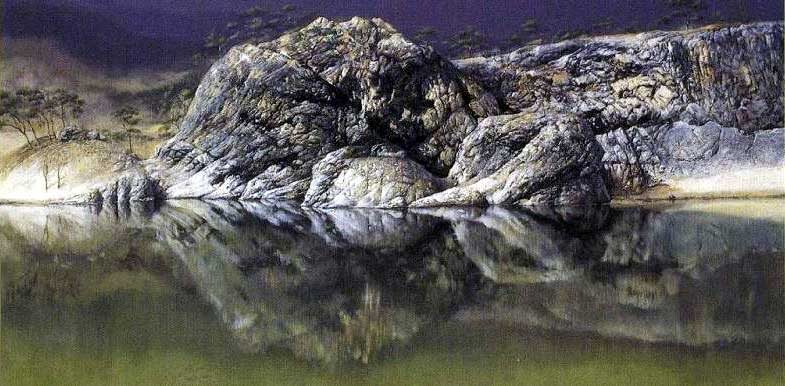
\includegraphics[width=.9\textwidth]{./img/hidden-woman-child.jpg}
        }
        \only<2>{
            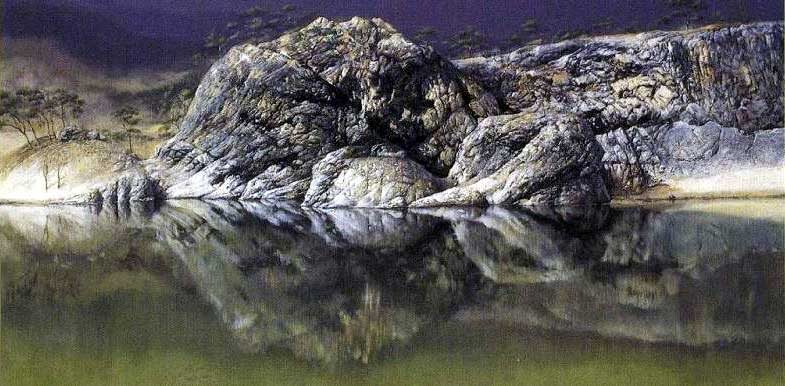
\includegraphics[width=.8\textwidth,angle=-90]{./img/hidden-woman-child.jpg}
        }
        \only<3>{
            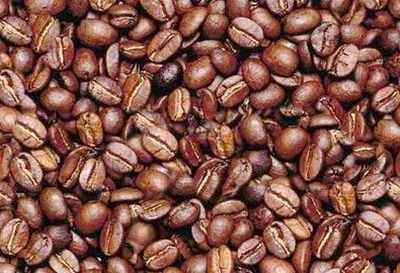
\includegraphics[width=.8\textwidth]{./img/coffee-illusion.jpg}
        }
    \end{center}
}

\frame{
    \begin{center}
        \begin{quote}
            How do you prove a mathematical theorem?
        \end{quote}
    \end{center}
}

\frame{
    \begin{center}
        \(\sqrt{2}\) is irrational.
    \end{center}
}

\frame{
    \[
        |\text{ASM}(n)|=\prod_{k=0}^{n-1}\frac{(3k+1)!}{(n+k)!}
    \]
}

\frame{
    \begin{itemize}
        \item Focus on quantity of ideas;
        \item Welcome unusual ideas;
        \item Combine, improve and modify;
        \item Suspend judgement.
    \end{itemize}
}

\frame{
    \begin{center}
        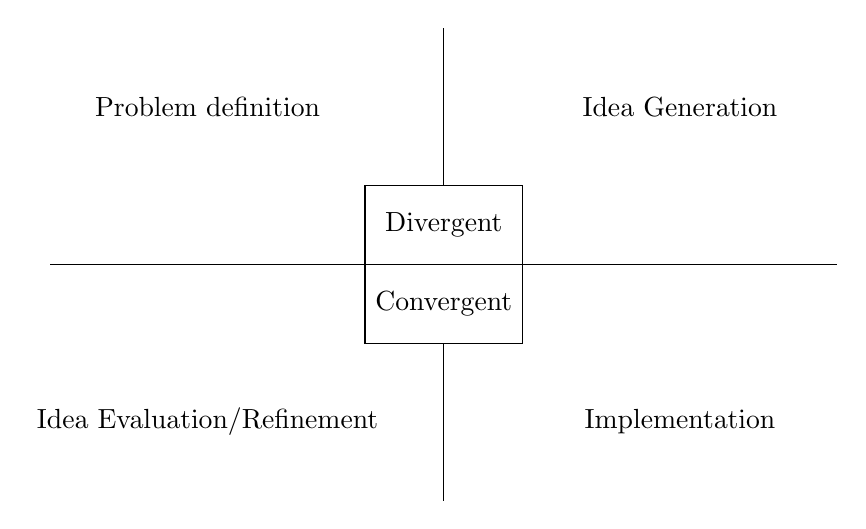
\begin{tikzpicture}
            \draw (0,-3) -- (0,-1);
            \draw (0,3) -- (0,1);
            \draw (-5,0) -- (5,0);
            \draw (-1,-1) rectangle (1,1);
            \node at (0,.5) {Divergent};
            \node at (0,-.5) {Convergent};
            \node at (-3,2) {Problem definition};
            \node at (3,2) {Idea Generation};
            \node at (-3,-2) {Idea Evaluation/Refinement};
            \node at (3,-2) {Implementation};
        \end{tikzpicture}
    \end{center}
}

\frame{
    \frametitle{What your company does and why?}
        \begin{itemize}
            \item Aims/Objectives
                \begin{itemize}
                    \item What does the business hope to achieve?
                    \item Create \textbf{S}pecific, \textbf{M}easurable, \textbf{A}chievable, \textbf{R}ealistic, \textbf{T}ime bound objectives.
                \end{itemize}
            \item Creating value
                \begin{itemize}
                    \item What are the main features and benefits?\\

                        \textit{Think: durability, low price, portability, long lasting usage, affordable, can it be used anywhere?}

                    \item Consider the environment in which you are to operate.\\

                        \textit{Think: economy, regulation, legislation, funding, is there a report highlighting the need? }

                \end{itemize}
        \end{itemize}
}

\frame{
    \begin{center}
            \huge{USP}
    \end{center}
}

\frame{
    \begin{center}
        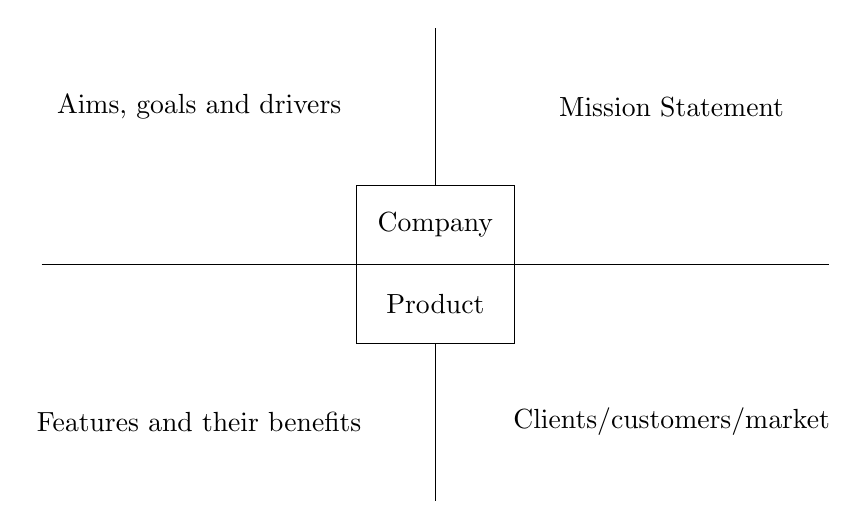
\begin{tikzpicture}
            \draw (0,-3) -- (0,-1);
            \draw (0,3) -- (0,1);
            \draw (-5,0) -- (5,0);
            \draw (-1,-1) rectangle (1,1);
            \node at (0,.5) {Company};
            \node at (0,-.5) {Product};
            \node at (-3,2) {Aims, goals and drivers};
            \node at (3,2) {Mission Statement};
            \node at (-3,-2) {Features and their benefits};
            \node at (3,-2) {Clients/customers/market};
        \end{tikzpicture}
    \end{center}
}

\end{document}
